\documentclass[english,seminar,headertitle]{lecture}
\usepackage{tikz}

\title{Advanced classical mechanics}
\subtitle{Mechanics of a system of particles}
\shorttitle{System of particles}
\ccode{16MSPAH101}
\subject{Classical mechanics}
\speaker{V.H. Belvadi}
\spemail{vh@belvadi.com}
\author{}
\email{}
\flag{}
\season{Summer 2017}
\date{}{}{}
\dateend{}{}{}
\conference{}
\place{St Philomena's College}
\attn{}
\morelink{vhbelvadi.com/teaching}

\begin{document}
\noindent Physics as we know it began with Newton's work on what is now called classical mechanics. However the Newtonian approach is hardly the only method of studying classical phenomena. Joseph Louis Lagrange, in 1788, and William Rowan Hamilton, in 1833, reformulated Newtonian mechanics into two formalisms that are now called Lagrangian and Hamiltonian mechanics respectively. Think of these as three different but equivalent methods of solving the same classical problems. This paper will focus on the works of Lagrange and Hamilton and calls for a divagation from the Newtonian approach that we are so familiar with.
%
\section{Conservation of momenta}

\subsection{Linear momentum}\label{sec:linear-momentum}
%
We start by establishing a fundamental law of physics, the law of conservation of momentum, that states that linear and angular momenta in a system are conserved so long as no net force acts on it.

Recall Newton's second law which tells us that the rate of change of momentum is force. In considering the forces involved in a system of point particles notice that not only can there be some external force $\mathbf{F}_i^{(e)}$ on the $i^\textrm{th}$ particle but there may also be an internal force $\mathbf{F}_{ji}$ on the same $i^\textrm{th}$ particle but this time due to some other $j^\textrm{th}$ particle within the system. Of course when $i = j$ we have $\mathbf{F}_{ii} = 0$ since a point particle exerts no force on itself. Newton's second law for a system of particles is therefore written as
\begin{equation}
\sum_j\mathbf{F}_{ji} + \mathbf{F}_i^{(e)}= \dot{\mathbf{p}}_i \label{eq:newton-second-single-particle}
\end{equation}%
where $\mathbf{\dot{p}}_i$ is the linear momentum of the $i^\textrm{th}$ particle and we have summed $\mathbf{F}_{ji}$ over all other particles in the system since any number of them may exert a force on the $i^\textrm{th}$ particle. We can also extend this to \textit{all} the particles in our system by writing
\begin{equation}
\sum_{j,i \neq j}\mathbf{F}_{ji} + \sum_i\mathbf{F}_i^{(e)} = {\textrm{d}^2 \over \textrm{d}t^2} \sum_i m_i\mathbf{r}_i \label{eq:newton-second-multi-particle}
\end{equation}%

To reduce the left-hand side notice that the first term introduces pairs of $\mathbf{F}_{ij}$ and $\mathbf{F}_{ji}$ which are pairs of forces where one is exerted by the $j^\textrm{th}$ particle on the $i^\textrm{th}$ particle and another by the $i^\textrm{th}$ particle on the $j^\textrm{th}$ particle. Newton's third law tells us that these two forces are in fact equal and opposite, so all such pairs of forces cancel out, sending the first term to zero.

The second term on the left-hand side gives the external force per particle summed over all particles which is nothing but the total external force $\mathbf{F}^{(e)}$ acting on the system.

The right-hand term gives the momentum of the $i^\textrm{th}$ particle in terms of its mass and position vector. This can be reduced using the equation of the centre of mass of the entire system 
\begin{equation}
\sum_i m_i \mathbf{R} = \sum_i m_i\mathbf{r}_i \label{eq:com}
\end{equation}%
where $\mathbf{R}$ is the position vector of the centre of mass. For simplicity if we redefine $\sum_i m_i = M$, the total mass of the system, we end up with $$\mathbf{F}^{(e)} = M {\textrm{d}^2\mathbf{R}\over\textrm{d}t^2}$$

This tells us that a system of particles moves under the action of a force\margintext{As we established earlier, although internal forces exist they have no influence on the system as a whole so long as Newton's third law remains valid.} as though only a net external force existed and it was acting on the total mass of the system concentrated at the centre of mass. In other words, the total linear momentum of the system given by
\begin{equation}
\mathbf{P} = M \textrm{d}\mathbf{R}/\textrm{d}t
\end{equation}%
is conserved when $\mathbf{F}^{(e)} = 0$ since, under this condition, $\mathbf{R}$ does not change with time. Verbally we state this as the \textbf{law of conservation of linear momentum}: \textit{When no external force acts on a system its total linear momentum is conserved}.

Remember, though, that for momentum to be conserved, Newton's third law (sometimes called the \textbf{weak law of action and reaction}) must be valid. Newton's third law \textit{can} be broken \cite{ivlev} when a system is out of equilibrium---these are called nonreciprocal reactions. As we will see in the next section, making sure this law stays valid is important for conserving angular momentum too. We will soon encounter this law in a slightly different form.
%
\subsection{Angular momentum}
%
Arguments similar to those in \ref{sec:linear-momentum} can be used to prove the conservation of angular momentum as well. The angular momentum of the $i^\textrm{th}$ particle in a system is given by $\mathbf{r}_i \times \mathbf{p}_i$ where the terms are as explained before. Here,
\begin{align*}
{\textrm{d}\over\textrm{d}t} (\mathbf{r}_i \times m\mathbf{v}_i)
&= \mathbf{v}_i \times m\mathbf{v}_i + \mathbf{r}_i \times m{\textrm{d}\mathbf{v}_i\over\textrm{d}t} \\
&= \mathbf{r}_i \times m{\textrm{d}\mathbf{v}_i\over\textrm{d}t} = \mathbf{r}_i \times \mathbf{\dot{p}}_i
\end{align*}

Combining this with eq. (\ref{eq:newton-second-single-particle}) we get
\begin{align*}
	\sum_{j,i\neq j} (\mathbf{r}_i \times  \mathbf{F}_{ji}) + \sum_i (\mathbf{r}_i \times \mathbf{F}_i^{(e)}) &= \sum_i (\mathbf{r}_i \times \mathbf{\dot{p}}_i) \\
	&= \sum_i {\textrm{d}\over\textrm{d}t} (\mathbf{r}_i \times \mathbf{p}_i) = \mathbf{\dot{L}}
\end{align*}
where $\mathbf{L}$ is the angular momentum.

The term $\sum_{j,i\neq j} (\mathbf{r}_i \times  \mathbf{F}_{ji})$ is, as we saw in \ref{sec:linear-momentum}, pairs of forces and they now look like $\mathbf{r}_i \times \mathbf{F}_{ji} = - \mathbf{r}_j \times \mathbf{F}_{ij}$ or simply $(\mathbf{r}_i - \mathbf{r}_j) \times \mathbf{F}_{ji}$ (since $\mathbf{F}_{ji} = -\mathbf{F}_{ij}$) so long as Newton's third law is valid. The vector $(\mathbf{r}_i - \mathbf{r}_j)$ is a separation vector going to the $i^\textrm{th}$ particle from the $j^\textrm{th}$ particle which we shall represent as $\mathbf{r}_{ij}$ to finally write $\mathbf{r}_{ij} \times \mathbf{F}_{ji}$.

Notice that if the equal and opposite internal forces between two particles is also along the lines joining them, i.e. when the separation vector makes a zero or 180 degree angle with the position vectors, the $\mathbf{r}_{ij} \times \mathbf{F}_{ji}$ terms all go to zero. We are left with just the external torque $\sum_i (\mathbf{r}_i \times \mathbf{F}_i^{(e)}) = \mathbf{N}^{(e)}$ (say) which now leaves us with
\begin{equation}
{\textrm{d}\mathbf{L}\over\textrm{d}t} = \mathbf{N}^{(e)} \label{eq:L-conservation}
\end{equation}%
which says that the angular momentum is a constant so long as $\mathbf{F}^{(e)} = 0$, or, verbally, the \textbf{law of conservation of angular momentum}: \textit{When the external torque applied on a system is zero its angular momentum is a constant in time}.

In both cases for conservation keep in mind that our momenta are vectors, i.e. $\mathbf{p} \equiv p_x + p_y + p_z$ and likewise for $\mathbf{L}$. As a result, if $N_x^{(e)} = 0$ then $L_x^{(e)} = 0$ as well even though $N_x^{(e)}$ and $N_x^{(e)}$ may not be zeroes.

For angular momentum to be conserved not only must the weak law of action and reaction be satisfied but so too should a second condition: the action and reaction forces between two masses must both act along the line joining those two masses. This is called the \textbf{strong law of action and reaction} and forces that obey this law are called \textbf{central forces}.

\begin{figure}
\centering
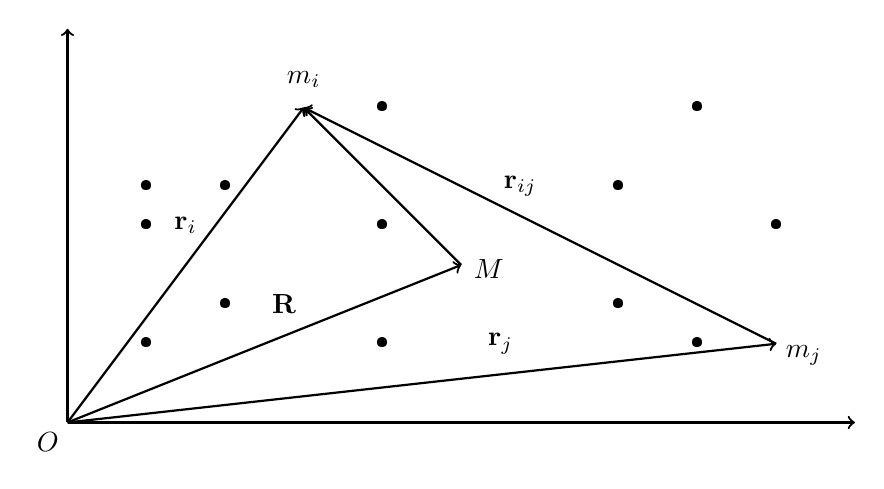
\begin{tikzpicture}
	\draw[->,thick] (0,0) -- (0,5);
	\draw[->,thick] (0,0) -- (10,0);
	\draw[->,thick] (0,0) -- (5,2);
	\draw[->,thick] (0,0) -- (3,4);
	\draw[->,thick] (0,0) -- (9,1);
	\draw[->,thick] (5,2) -- (3,4);
	\draw[->,thick] (9,1) -- (3,4);
	
	\node at (2.75,1.5){$\mathbf{R}$};
	\node at (1.5,2.5){$\mathbf{r}_i$};
	\node at (5.5,1){$\mathbf{r}_j$};
	\node at (5.75,3){$\mathbf{r}_{ij}$};
	\node at (5.35,1.95){$M$};
	\node at (9.35,0.85){$m_j$};
	\node at (3,4.35){$m_i$};
	\node at (-0.25,-0.25){$O$};
	
	\foreach \Point in {(2,1.5), (1,1), (2,3), (1,2.5), (1,3), (8,4), (7,3), (9,2.5), (4,1), (4,4), (8,1), (7,1.5), (4,2.5)}{
    \node at \Point {\textbullet};
}
\end{tikzpicture}
	\caption{A system of many point particles.}\label{fig:com}
\end{figure}

So much for conserving angular momentum, but what is the angualar momentum in the first place? We know that the total angular momentum of our many-particle system is
\begin{equation}
\mathbf{L} = \sum_i \mathbf{r}_i \times \mathbf{p}_i \label{eq:L-basic}
\end{equation}%
where $\mathbf{r}_i$ is the radius vector from the origin to the $i^\textrm{th}$ particle and $\mathbf{p}_i$ is the linear momentum of that particle. Suppose, as before, that $\mathbf{R}$ is the radius vector to the centre of mass of the system; we now have a separation vector $\mathbf{r}_i'$ between $\mathbf{R}$ and $\mathbf{r}_i$ going from the centre of mass to the $i^\textrm{th}$ particle. That is to say, $\mathbf{R} + \mathbf{r}_i' = \mathbf{r}_i$ is then the vector sum describing the three position vectors.

In terms of velocities this simply means that the equation $\mathbf{v} + \mathbf{v}_i' = \mathbf{v}_i$ describes the velocities of the centre of mass, the velocity of the $i^\textrm{th}$ particle with respect to the centre of mass, and the velocity of the $i^\textrm{th}$ particle itself respectively. All of these vectors have been represented in fig. \ref{fig:com} above with the same notation.

This leaves us with eq. (\ref{eq:L-basic}) written in terms of the centre of mass as
\begin{align}
	\mathbf{L} &= \left[ \sum_i \mathbf{R} \times m_i\mathbf{v}_i \right] + \left[ \sum_i \mathbf{r}_i' \times m_i\mathbf{v}_i \right]\nonumber \\
	&= \left[ \sum_i \mathbf{R} \times m_i\mathbf{v} + \mathbf{R} \times {\textrm{d}\over\textrm{d}t} \sum_i m_i\mathbf{r}_i' \right] + \left[ \sum_i \mathbf{r}_i' \times m_i\mathbf{v} + \sum_i \mathbf{r}_i' \times m_i\mathbf{v}_i' \right] \nonumber \\
\Rightarrow \mathbf{L} &= \mathbf{R} \times M \mathbf{v} + \sum_i \mathbf{r}_i' \times \mathbf{p}_i' \label{eq:L-full}
\end{align}
where we have first used the expression for $\mathbf{r}_i$ and then that for $\mathbf{v}_i$ to expand eq. (\ref{eq:L-basic}) and, further, we realise that the second and third terms on the right-hand side, containing the term $\sum m_i r_i'$, vanish since they define a radius vector from the centre of mass to itself (compare this term with eq. (\ref{eq:com}) and fig. \ref{fig:com} to see why this is so) thereby nullifying themselves.

Equation (\ref{eq:L-full}) tells us is that the angular momentum of a system of particles about an arbitrary reference point $O$ is the angular momentum of its motion as if \textit{concentrated at} the centre of mass plus the angular momentum \textit{about} the centre of mass itself. If, however, the centre of mass of the system is at rest with respect to the arbitrary reference point then $\mathbf{R} \times M\mathbf{v} = 0$ since there is no motion with respect to that point and only the motion about the centre of mass, given by the second term, remains, promptly giving us eq. (\ref{eq:L-basic}) back.
%
\section{Basic ideas of analytical mechanics}
%
The foundations of Lagrangian mechanics are the kinetic and potential energies involved in a system. In fact it is this use of scalar quantities that characterises this approach to studying the mechanics of bodies, sometimes also known as \textbf{analytical mechanics}\margintext{The word `analytical' in analytical mechanics refers not to analysis but to the use of infinitesimal calculus in solving physical and mathematical problems.}, as opposed to the vectorial approach taken by Newtonian mechanics. Now and for the rest of this course we will maintain the notation $T$ for kinetic energy and $V$ for potential energy.

Having established that momenta in a system remain constant with time so long as no external force acts on the system, we will now examine $T$ and $V$. This will finally set the stage for our discussions of Lagrangian mechanics. But before we begin that discussion it is worth taking a moment to understand how analytical mechanics varies from Newtonian mechanics.

Most people only they of Newtonian mechanics think of when the word `mechanics' is brought up in a discussion; but analytical mechanics is an equally interesting, at times more convenient method of studying a system. Generally, if a phenomenon can be analysed using the Newtonian method (identify forces, associate vectors with the system etc.) it can also be analysed using Lagrangian and Hamiltonian methods. Further, analytical mechanics provides a sort of bridge between classical mechanics and quantum mechanics. Here is a quick overview \cite{lanczos} of the two approaches:
\begin{enumerate}
	\item Newtonian mechanics considers individual parts of a system; analytical mechanics considers the system as a whole (hence our discussion of a system of many particles rather than of individual particles).
	\item Newtonian mechanics identifies forces acting on individual parts of a system; analytical mechanics uses a single \textbf{work function} (often energy).
	\item Forces within a system have to be maintained, particularly with respect to the relative positions of co\"{o}rdinates, while solving a problem vectorially; analytical mechanics does not require any knowledge of the forces maintaining co\"{o}rdinate positions within a system.
	\item Developing equations of motion using the Newtonian approach requires knowledge of several vectorial parameters; doing so analytically relies solely on a single, unified principle based on a quantity called `action' (which we will discuss soon in coming lectures).
\end{enumerate}
We will discuss more specific ideas about analytical mechanics, particularly configuration space, generalised co\"{o}rdinates etc., as we go. For now this brief introduction should suffice; we shall turn our attention towards describing $T$ and $V$ for our system as promised.
%
\section{Energies and rigid bodies}
\subsection{Kinetic energy}
%
For now think of the configuration of a system as a set of variables that define the system at any point; this could be position, velocity etc. Knowing all these parameters is like knowing the \textit{configuration} of a system. During the occurrence of a phenomenon some of these parameters may change taking the system to another configuration, i.e. giving us a new set of variables that describe the same system.

We can show quite easily that the work--energy relationship remains the one we are familiar with from Newtonian mechanics (and this should be no surprise either since we are not trying to break Newton's laws down). Say we go from configuration 1 to configuration 2. We know that the work done in the process depends on the force applied and the displacement it brings about:
$$
W_{12} = \sum_i \int_1^2\mathbf{F}_i \cdot \textrm{d}\mathbf{s}_i
$$
And from eq. (\ref{eq:newton-second-multi-particle}) we know the total force $\mathbf{F}_i$ on our system to be the sum of two forces:
\begin{equation}
W_{12} = \sum_i \int_1^2 \mathbf{F}_i^{(e)} \cdot \textrm{d}\mathbf{s}_i + \sum_{j,i\neq j} \int_1^2 \mathbf{F}_{ji} \cdot \textrm{d}\mathbf{s}_i \label{eq:W12}
\end{equation}
Consider the term $\sum_i \int_1^2\mathbf{F}_i \cdot \textrm{d}\mathbf{s}_i$ which we can expand into a familiar form:
$$
\sum_i \int_1^2 \left( \mathbf{F}_i \right) \cdot \left( \textrm{d}\mathbf{s}_i \right) = \sum_i \int_1^2 \left( m_i\mathbf{\dot{v}}_i \right) \cdot \left( \mathbf{v}_i \textrm{d}t \right) = \sum_i \int_1^2 \textrm{d}\left( {1\over 2} m_i \mathbf{v}_i^2 \right)
$$
where we know that the last term in parentheses
\begin{equation}
T = {1\over 2} \sum_i m_i \mathbf{v}_i^2 \label{eq:T-basic}
\end{equation}%
is the kinetic energy $T$ of the system. In other words, the work done in going from configuration 1 to configuration 2 can still be written in a familiar form as the difference between the kinetic energies of the system at those two configurations, i.e. $W_{12} = T_2 - T_1$.

Knowing that $\mathbf{r}_i = \mathbf{r}_i' + \mathbf{R}$ we can expand eq. (\ref{eq:T-basic}) as
\begin{align*}
T &= {1 \over 2} \sum_i m_i (\mathbf{v} + \mathbf{v}_i')(\mathbf{v} + \mathbf{v}_i') \\
&= {1 \over 2} \sum_i m_i v^2 + {1 \over 2} \sum_i m_i v_i'^2 + \mathbf{v} \cdot {\textrm{d}\over\textrm{d}t} \left( \sum_i m_i r_i' \right)
\end{align*}%
where, for the same reasons as with eq. (\ref{eq:L-full}), the last term vanishes giving us
\begin{equation}
	T = {1 \over 2} \sum_i m_i v^2 + {1 \over 2} \sum_i m_i v_i'^2 \label{eq:T}
\end{equation}%
a more proper form of the kinetic energy of a system of many particles which looks remarkably similar to eq. (\ref{eq:L-full}) for angular momentum: the total kinetic energy is the kinetic energy calculated as if all the mass were concentrated at the centre of mass plus the kinetic energy of motion about the centre of mass.
%
\subsection{Potential energy}
%
The same reasoning can be expanded to compute the potential energy as well. Specifically we will return our focus to eq. (\ref{eq:W12}) where the external force can be expressed as the negative gradient of a scalar potential\margintext{Any conservative force can be expressed this way---proofs are available aplenty, look it up. The more important note here is that we are demanding that the external forces acting on the system be conservative.} as
$$
\sum_i \int_1^2 \mathbf{F}_i^{(e)}\cdot\textrm{d}\mathbf{s}_i = - \sum_i \int_1^2 \nabla_i V_i \cdot \textrm{d}\mathbf{s}_i = - \sum_i V_i \Bigr|_1^2
$$
where $V$ is the potential energy associated with the system and $\nabla_i$ refers to differentiation with respect to $\mathbf{r}_i$ of the $i^\textrm{th}$ particle (and the integral and the del operator cancel each other out).

In the same manner the force $\mathbf{F}_{ij}$ on any $i^\textrm{th}$ particle can be associated with a potential $V_{ij}$ which is a function of the separation between the $i^\textrm{th}$ and $j^\textrm{th}$ particle, i.e. $V_{ij} \equiv V_{ij}(| \ \mathbf{r}_i - \mathbf{r}_j \ |)$. Therefore the pair of forces $\mathbf{F}_{ij}$ and $-\mathbf{F}_{ji}$ are equal (and opposite, as evinced by the signs) and, in terms of their associated potentials, may be expressed as $-\nabla_i V_{ij}$ and $\nabla_j V_{ij}$ respectively.

Now the second term in eq. (\ref{eq:W12}) can be written in terms of the sum of pairs of potentials with each pair described by
$$
\sum_{j, i\neq j}\int_1^2 \mathbf{F}_{ji}\cdot\textrm{d}\mathbf{s}_i = {1\over 2} \sum_{j, i \neq j} \int_1^2 \left( \nabla_i V_{ij} \cdot \textrm{d}\mathbf{s}_i + \nabla_j V_{ji} \cdot \textrm{d}\mathbf{s}_j \right)
$$
where the $1/2$ arises because, in considering pairs and summing over all $i$ and $j$ we are including each particle twice.

The term $\nabla_i V_{ij}$ can be expressed as $-\nabla_j V_{ij}$ equivalently. Suppose we represent this as $\nabla_{ij} V_{ij}$ we end up with a single term expressing each pair:
$$
\int \nabla_{ij} V_{ij} \cdot \textrm{d}\mathbf{r}_{ij}
$$
where $\mathbf{r}_{ij}$ is a representative term for $\textrm{d}\mathbf{s}_i - \textrm{d}\mathbf{s}_j = \textrm{d}\mathbf{r}_i - \textrm{d}\mathbf{r}_j$. As a result the internal work term from eq. (\ref{eq:W12}) becomes
\begin{align*}
\sum_{j, i\neq j}\int_1^2 \mathbf{F}_{ji}\cdot\textrm{d}\mathbf{s}_i &= {1\over 2} \sum_{j, i \neq j} \int_1^2 \nabla_{ij} V_{ij} \cdot \textrm{d}\mathbf{r}_{ij} \\
&= {1 \over 2} \sum_{j, i \neq j} V_{ij} \Bigr|_1^2
\end{align*}%

This is the internal potential energy of our system. Using this and the external potential energy $\sum_i V_i$ we can define the total potential energy
\begin{equation}
	V = \sum_i V_i + {1 \over 2} \sum_{j, i\neq j} V_{ij} \label{eq:V}
\end{equation}%
of our system such that from this equation and eq. (\ref{eq:T}) we end up with the total energy of our system $T+V$ which---analogous to the Newtonian, individual particle case---is a conserved quantity. This observation, called the \textbf{law of conservation of energy}, is among the most important laws in physics.

The second term in eq. (\ref{eq:V}) is often not zero since all bodies have some internal energy. Further, it may not be a constant either. However, when this internal potential energy is a constant we say the body is a \textbf{rigid body}.

To be specific a rigid body\margintext{The idea of rigid bodies is an important one and we will spend quite a bit of time studying them over the length of this course.} is one where \textit{the magnitude of separation or distance $r_{ij}$ between two of its constituent particles is a constant}. Because of this any change in $r_{ij}$, given by $\textrm{d}\mathbf{r}_{ij}$ cannot be along the line joining the two bodies, i.e. it cannot be along $\mathbf{r}_{ij}$, since we said the separation is a constant; that is to say $\textrm{d}\mathbf{r}_{ij}$ can only be perpendicular to $\mathbf{r}_{ij}$ and, by extension, to $\mathbf{F}_{ij}$. Therefore the second term in eq. (\ref{eq:W12}) goes to zero (cosine of a perpendicular angle) telling us that the internal forces in a rigid body do no work.
%
\begin{thebibliography}{1}
	\bibitem{lanczos}
	Lanczos, Cornelius, \textit{The Variational Principles of Mechanics}, University of Toronto Press, 1949.
	
	\bibitem{goldstein}
	Goldstein, H., Poole, C., Safko, J., \textit{Classical mechanics}, 3rd edition, Addison Wesley, 2000.
	
	\bibitem{ivlev}
	Ivlev, A.V., Bartnick, J., Heinen, C. et al., \textit{Statistical Mechanics where Newton's Third Law is Broken}, Phys. Rev. X 5, 011035, 26 March 2015.
\end{thebibliography}

































\end{document}